\documentclass[9pt,technote]{IEEEtran}
 
\usepackage[T1]{fontenc}
\usepackage[utf8]{inputenc}
\usepackage{cite}
\usepackage{newtxtext,newtxmath}
\usepackage{tablefootnote}
\usepackage{graphicx}
\title{Linear Regression}
\author{
	Gian Marco Balia\\
	Robotic Engineering - University of Genoa\\
	s4398275@studenti.unige.it
}
 
\begin{document}
	\maketitle
	\begin{abstract}
Linear regression is a statistical technique used to model the relationship between a dependent variable and one or more independent variables by fitting a linear equation to observed data. Widely used across fields like economics, biology, and engineering, linear regression is valued for its simplicity and interpretability in predictive modeling. While it assumes a linear relationship and is sensitive to outliers, enhancements like regularization and multivariate approaches improve its robustness. This paper reviews the basics of linear regression, its applications, and methods to strengthen model accuracy.
	\end{abstract}
	\begin{IEEEkeywords}
Linear regression, multivariable, mean squared error
	\end{IEEEkeywords}
	\section{Introduction}
Linear regression is a useful tool for predicting a quantitative response, is still a useful and widely used statistical learning method \cite{james2023linear}.
In essence, it aim to predict a continuous target variable by finding the best-fitting line through the data points, minimizing the distance (or error) between the predicted values and the actual data points. This is achieved by adjusting the slope and intercept of the line to reduce the error, typically measured by a cost function such as Mean Squared Error ($MSE$) \cite{Montgomery}.
Linear regression is widely used not only for predictive analysis but also as a diagnostic tool to understand relationships between variables, particularly in areas like economics, biology, and social sciences. It serves as a baseline in machine learning to assess more complex models, and although it has limitations \cite{James}.
 
	\section{Material and methods}
 
	\subsection{Data processing}
There where analysed two different datasets:
	\begin{itemize}
		\item \textit{turkish-se-SP500vsMSCI} contains, in the first column, historical data on the returns of the S\&P 500 index (USA) and, in the second, the MSCI Europe index, representing the U.S. and European stock markets.
		\item \textit{mtcarsdata-4features} contains four features from the mtcars dataset, which collects data on various car models. The four main variables include \textit{mpg} (Miles Per Gallon, as an indicator of fuel efficiency), \textit{weight} (vehicle weight), \textit{hp} (horsepower), and \textit{disp} (engine displacement). This dataset is used to analyze how a car’s mechanical characteristics affect fuel consumption.
	\end{itemize}
Each dataset is initialized to store training and test subsets. The data is randomly shuffled before splitting into training and test subsets. For the Turkish dataset, ten subsets are created for cross-validation purposes, while the MTK data is split into training (5\%) and test (95\%) sets. To show the difference, is selected data from the beginning and end of the Turkish dataset rather than random samples, as nearby data points are often more similar.
 
	\subsection{Linear Regression Model}
The presented Linear Regression Model, works in two different methods. For the Turkish dataset the LRM's efficiency is evaluated using ten random subsets, each one a different $10\%$ of the dataset (Figure \ref{fig::turkish_with_intercept}). Instead, with the MTK dataset the model is implemented in two variables and multivariable linear regression represented in Figures \ref{fig::mkt2dim_without_intercept}, \ref{fig::mkt2dim_with_intercept}, and \ref{fig::mkt4dim_with_intercept}. Another evaluation taken to account is the applications of a intercept value.
		\subsubsection{Turkish dataset}
		is shuffled and split in two subsets (one for training and one for testing). The training's subsets takes each the $5\%$ of the entire dataset, meanwhile the testing's subsets the remainder $95\%$.
		\subsubsection{MTK dataset}
		 is analyzed in two different ways: first, considering only the first two columns (\textit{weight} and \textit{mpg}), and then considering all four columns (\textit{disp}, \textit{hp}, \textit{weight}, and \textit{mpg}) where there is applied a multidimensional linear regression. This allows us to evaluate the impact of additional features on the linear regression model.\\\\
		The performance of the linear regression model is also evaluated in two different scenarios: with and without intercept.
			
		\begin{figure}
			\centering
  			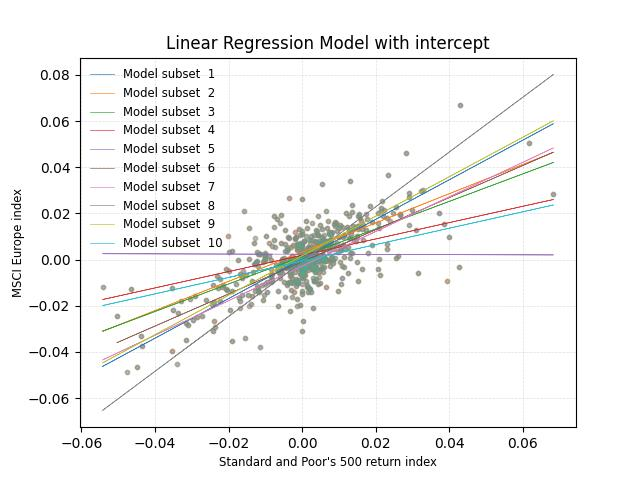
\includegraphics[width=1\linewidth]{figures/turkish_with_intercept.jpg}
  			\caption{Graphical representation of the model trained on ten subsets with interception, each corresponding to $5\%$ of the Turkish dataset. In the background are visualized the corrispective test subsets ($95\%$ of the dataset).}
  			\label{fig::turkish_with_intercept}
		\end{figure}

		\begin{figure}
			\centering
  			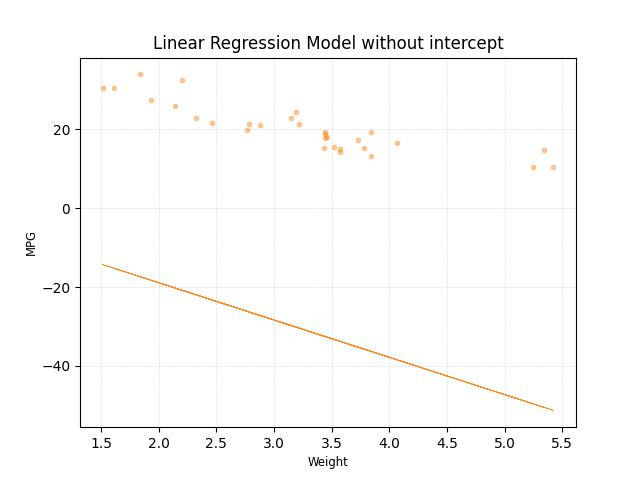
\includegraphics[width=1\linewidth]{figures/mkt2dim_without_intercept.jpg}
  			\caption{Graphical representation of the model trained without interception, which corresponds to $5\%$ of the MTK dataset. In the background is visible the test subset ($95\%$ of the dataset).}
  			\label{fig::mkt2dim_without_intercept}
		\end{figure}
		
		\begin{figure}
			\centering
  			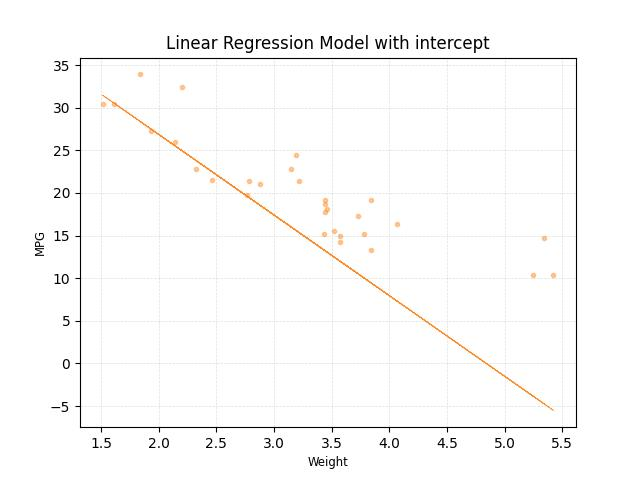
\includegraphics[width=1\linewidth]{figures/mkt2dim_with_intercept.jpg}
  			\caption{Graphical representation of the model trained with interception, which corresponds to $5\%$ of the MTK dataset. In the background is visible the test subset ($95\%$ of the dataset).}
  			\label{fig::mkt2dim_with_intercept}
		\end{figure}
		
		\begin{figure}
			\centering
  			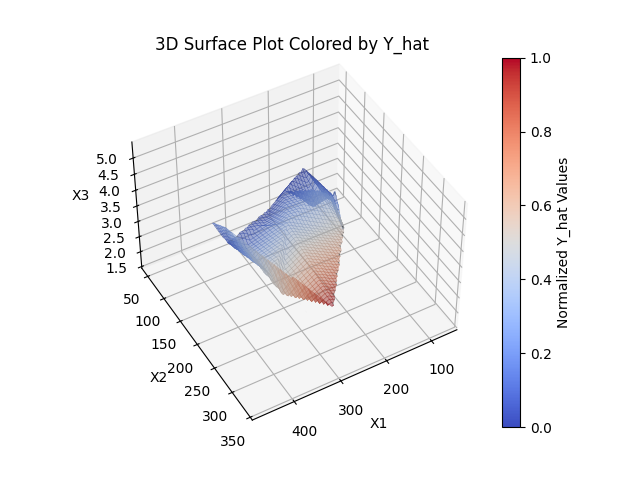
\includegraphics[width=1\linewidth]{figures/mkt4dim_with_intercept.png}
  			\caption{Graphical representation in fourth dimensional representation, where the fourth one is the predicted output. The model, trained with interception, corresponds to $5\%$ of the MTK dataset.}
  			\label{fig::mkt4dim_with_intercept}
		\end{figure}	
		
	Linear regression use the concept of the mathematical relation  
		\begin{equation*}
			y = \beta_0 + \beta_1 x
		\end{equation*}
	where  $y$  is the dependent variable,  $x$  is the independent variable, $\beta_0$  is the intercept,  $\beta_1$  is the slope of the line \cite{james2021LinearRegression}. But, unless the independent and dependent variables are describable as only two point in the domain the previous relation can be found only introducing an error term $\varepsilon$.
		\begin{equation}
			y = \beta_0 + \beta_1 x + \varepsilon
		\end{equation}
	The intercept $\beta_0$ in linear regression is the value of $y$ when all predictors $x$ are zero. Including the intercept allows the model to better fit the data, especially when it’s unrealistic to assume that $y = 0$ in the absence of independent variables, which forces the model to pass through the origin. It is useful only if there are theoretical reasons for y to be zero when the predictors are zero.
	In linear regression, $\epsilon$ represents the \textit{model's error} or \textit{residual term} \cite{james2021LinearRegression}. Epsilon captures all the variations in $y$ that cannot be predicted by the independent variables used in the model.
	Mathematically, epsilon is the difference between the observed value of $y$ and the value predicted by the linear model:
	\begin{equation*}
		\varepsilon= y_{\tiny\text{observed}} - y_{\tiny\text{predicted}}
	\end{equation*}
	The $\varepsilon$ term is crucial because it highlights the model's limitations and suggests that, despite efforts to model the data, there will always be unpredictable elements or unconsidered factors that influence the outcome.

	Multivariable linear regression is an extension of simple linear regression and is used to model the relation between a dependent variable (or target) and two or more independent variables (or predictors).
	\begin{equation}
		y = X \mathbf w
	\end{equation}
	where $X$ are the independent variables represented by matrix form and $\mathbf w$ is the slope's vector. If it considered the intercept must be added a unit column at the beginning of the $X$ matrix. \\
	Another important point considered to implement the model is the computation of the pseudo-inverse in case of exceptions. In particular, the pseudo-inverse (which is a generalization of the matrix inverse, without the condition of invertibility) is computed when, during the computation of the gradient, the matrix is not invertible. This means that the system of linear equations would not have solutions, and the pseudo-inverse is used to provide an approximate solution.
	\subsection{Model evaluation}
	\textit{Mean Squared Error} (MSE) is a key metric that quantifies the overall accuracy of the model. It is computed as the average of the squared differences between the observed values and the predicted values across all data points:
	\begin{equation}
		\text{MSE} = \frac{1}{n} \sum_{i=1}^{n} \varepsilon_i^2
	\end{equation}
	MSE is used as a \textit{loss function} to minimize the model error during the training, and it provides an aggregate measure of the prediction error across the dataset.
	
	\section{Results}
	From Figure \ref{fig::mkt2dim_without_intercept} and \ref{fig::mkt2dim_with_intercept} it is visible that, training the model with only two classes (i.e. \textit{weight} and \textit{mpg}) of the MTK data is notably different the use of the intercept. In the case of the training model without intercept the linear regression line of the predicted values does not intercept any point.
	In contrast, Figure \ref{fig::mkt4dim_with_intercept} presents challenges in obtaining readily comprehensible results. This may be attributed to the limited data set utilized for the regression analysis.
	 Analyzing the Turkish dataset, a median of $2.44 \cdot 10^{-4}$ was calculated for the mean squared error (MSE) obtained from the ten subsets. The first quartile was $2.20 \cdot 10^{-4}$, and the third quartile was $2.65 \cdot 10^{-4}$. These values were obtained for both cases analyzed: with and without the inclusion of an intercept.
	 		
	\section{Conclusion}
	In this report, we presented a linear regression analysis of two datasets: Turkish and MTK. Our results show that the linear regression model is able to capture the relationship between the variables in both datasets.
	For the Turkish dataset, we found that the model is able to explain a significant portion of the variance in the data, with a mean squared error (MSE) of $2.44 \cdot 10^{-4}$.
	For the MTK dataset, we analyzed the data in two different ways: considering only the first two columns (\textit{weight} and \textit{mpg}), and considering all four columns (\textit{disp}, \textit{hp}, \textit{weight}, and \textit{mpg}). Our results show that the model performs better when considering all four columns, with an MSE of $68.40$ and $225.28$. This suggests that the additional features in the dataset provide valuable information for predicting the target variable.
	Overall, our results demonstrate the effectiveness of linear regression in modeling the relationships between variables in these datasets. However, we also note that the MSE values are relatively small, indicating that the models may not be capturing all of the underlying patterns in the data.	
\bibliographystyle{IEEEtranS}
\bibliography{Bib.bib}

\end{document}